\documentclass[conference]{IEEEtran}
\usepackage{cite}
\usepackage{amsmath,amssymb,amsfonts}
\usepackage{algorithmic}
\usepackage{graphicx}
\usepackage{textcomp}
\usepackage{xcolor}
\usepackage{booktabs}
\usepackage{url}
\def\BibTeX{{\rm B\kern-.05em{\sc i\kern-.025em b}\kern-.08em T\kern-.1667em\lower.7ex\hbox{E}\kern-.125emX}}

\title{Auto-Decte: An LLM- and RAG-Assisted Human-in-the-Loop Document Intelligence System for Industrial Paper Forms}

\author{\IEEEauthorblockN{Anonymous Authors}
\IEEEauthorblockA{\textit{College of Computer Science and Electronic Engineering} \\
\textit{Hunan University}\\
Changsha, China \\
(anonymized for review)}}

\begin{document}
\maketitle

\begin{abstract}
Deploying large language models (LLMs) in high-stakes enterprise workflows is constrained less by model capability than by trust: suggestions must never silently become facts, every decision must be traceable to evidence, and the system must keep working when the model is unavailable. This paper presents Auto-Decte, a document intelligence system for industrial paper forms that operationalizes these constraints through a human-in-the-loop architecture. A fiducial-guided perception front end (QR/ArUco template recognition, perspective correction, per-cell digit and OMR recognition with an explicit ambiguity band) converts photographed paper forms into structured candidate values. An LLM suggestion adapter (DeepSeek, structured output) and a local vector similarity-retrieval module (RAG-style, read-only) assist reviewers, while a React review workbench makes the human the only source of truth: machine outputs are stored as append-only candidates, and only human confirmations or corrections become versioned, auditable records. A PWA front end with an offline outbox extends submission to in-plant mobile devices. The system is evaluated on end-to-end acceptance (389 public-snapshot tests, including the AI-off path and suggestion-isolation invariants), front-end recognition benchmarks (digit 93.9\% overall, 100\% on the printed font family; OMR 100\% correct outside the ambiguity band; QR 100\%; ArUco correction $\leq$0.34\,px), and per-image latency ($\approx$2.2\,s, QR search dominant).
\end{abstract}

\begin{IEEEkeywords}
LLM application, retrieval-augmented generation, human-in-the-loop, document intelligence, traceability, offline-first PWA
\end{IEEEkeywords}

\section{Introduction}
Foundation-model-assisted document processing is attractive for the long tail of paper-based workflows in small and medium plants, but its adoption in payroll-adjacent settings is blocked by a trust problem: an LLM that transcribes a digit wrong changes a worker's wage, and a retrieval system that injects a similar-looking historical record into a decision can silently corrupt it. Fully automatic pipelines are therefore unacceptable where errors carry financial consequences, yet purely manual digitization does not scale.

Auto-Decte addresses this with a human-in-the-loop architecture built on three principles: (i) \emph{machine outputs are candidates, never facts} --- the LLM adapter and every recognition stage emit candidates that a human must confirm or correct; (ii) \emph{the document is engineered} --- templates are generated with QR codes and ArUco fiducials so that perception is reliable rather than learned; (iii) \emph{everything is auditable} --- evidence is content-addressed, records are append-only versions, and every exported cell is back-traceable. The system is deployed as a working baseline at a bamboo-processing plant.

Contributions:
\begin{enumerate}
\item A human-in-the-loop document intelligence architecture for industrial paper forms, integrating a fiducial perception front end, an LLM suggestion adapter, and local similarity retrieval under a single ``candidates-only, human-confirmed'' trust boundary.
\item Trustworthy LLM/RAG integration mechanisms: suggestions are stored separately and can never mutate confirmed values; retrieval results are strictly read-only; the core pipeline runs and remains correct with the AI layer fully disabled (guarded by acceptance tests).
\item An engineered, interpretable perception front end --- synthetic-font template matching for digit cells and a fill-ratio OMR recognizer --- whose explicit ambiguity band routes borderline cells to humans instead of guessing.
\item An offline-capable mobile submission path (PWA + IndexedDB outbox + idempotency keys) that feeds the same review queue as scanned forms.
\item A deployment-motivated case study with end-to-end acceptance evidence and honest reporting of what remains unmeasured.
\end{enumerate}

\section{Related Work}
\textbf{Document OCR and layout analysis.} General document AI stacks (PP-OCRv3~\cite{ppocrv3}, LayoutLMv3~\cite{layoutlmv3}, Donut~\cite{donut}) target free-form documents with learned detection and recognition. Auto-Decte deliberately keeps learned layout models out of the critical path: system-generated templates make layout known exactly, so perception reduces to fiducial-guided cropping plus per-cell template matching; learned OCR remains a future extension for handwriting and Chinese text.

\textbf{LLM assistance and retrieval.} Retrieval-augmented generation and generative information-extraction surveys~\cite{llmgie,rag} and Local-First Software principles~\cite{localfirst} motivate two components: a read-only DeepSeek structured-output suggestion adapter and a local vector similarity index. The distinction from generic RAG is architectural: in Auto-Decte the model and the retriever are denied write access to facts by construction, and their outputs are versioned separately from records.

\textbf{Human-in-the-loop digitization.} HITL principles for high-stakes data (Budd et al.~\cite{budd}; drilling-report digitization~\cite{eage}) motivate the review workbench: machine outputs are append-only candidates, and every confirmed or corrected value is a versioned human decision with a before/after audit pair.

\textbf{Fiducial-based localization and OMR.} ArUco~\cite{aruco} and MILP dictionary markers~\cite{milp} provide geometric anchoring; existing OMR systems (e.g., SurveyNet~\cite{surveynet}) evaluate bulk mark recognition. Auto-Decte's distinguishing feature is the first-class ambiguity band: cells in the intermediate fill band are emitted with zero confidence and force review rather than a thresholded guess.

\textbf{Positioning.} Four decisions distinguish Auto-Decte from prior systems: (i) machine outputs --- from recognition and from the LLM alike --- are candidates, never facts; (ii) an explicit ambiguity band routes borderline cells to humans; (iii) full traceability --- SHA-256 evidence, versioned records, audit events, back-traceable exports; (iv) offline mobile submission integrated with the same review queue.

\section{System Overview}
Auto-Decte is a single-machine deployment: FastAPI (Python 3.11) backend, SQLite via SQLAlchemy 2.0 with Alembic migrations, React~18 + Vite front end, OpenCV for image operations, a DeepSeek client for structured-output suggestions, and a local vector index for similarity retrieval. Fig.~\ref{fig:arch} shows the pipeline stages.

\begin{figure}[t]
\centering
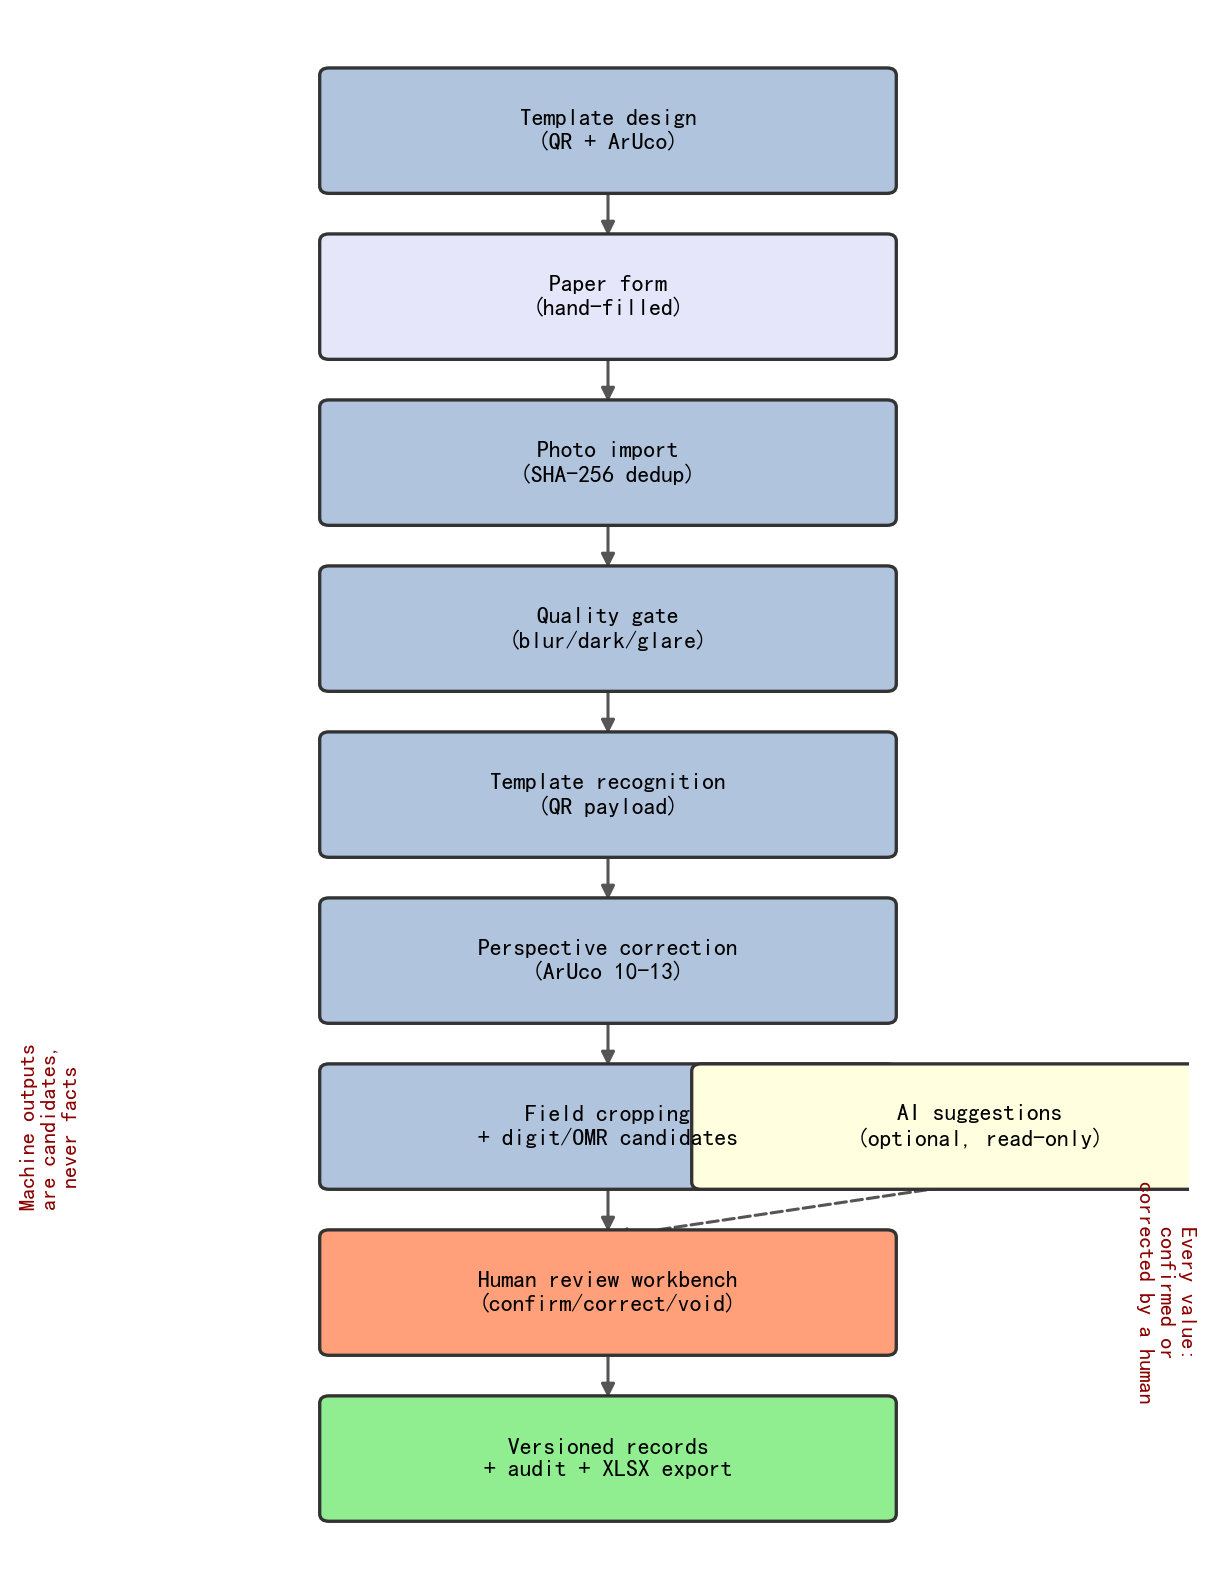
\includegraphics[width=0.42\columnwidth]{../figures/architecture.png}
\caption{End-to-end pipeline. Recognition and the LLM produce candidates and references; only human confirmations or corrections become facts.}
\label{fig:arch}
\end{figure}

The domain model separates immutable evidence, versioned form records (\texttt{RecordVersion}), append-only recognition attempts, isolated AI suggestions, read-only retrieval references, audit events, and export batches. Roles (operator, reviewer, finance, admin, auditor) gate every mutation.

\section{Template Design and Perception Front End}
Templates are designed and published inside the system (template center with versioning and draft canvas). Each published template renders a PDF/PNG with a QR code (template identity + version) and ArUco markers at known positions. Recognition is fiducial-first: a multi-region QR search classifies the form, four ArUco corner markers (IDs 10--13) map it to the canonical canvas, perspective correction aligns it, and per-field cells are cropped from the template definition. This makes identification and geometry deterministic and auditable.

\section{Field-Level Recognition with Confidence and Ambiguity}
\textbf{Digit cells.} Each cell is normalized to $48{\times}64$, binarized with Otsu thresholding, and matched against ten rendered synthetic-font templates (0--9) by normalized mean absolute difference. The recognizer reports the best digit, a distance-based confidence, and an \texttt{AMBIGUOUS} flag when the margin to the second-best template falls below $0.02$. Blank cells (ink ratio $<1\%$) are reported as blank rather than as a digit.

\textbf{Checkbox (OMR) cells.} Fill ratio in the cell interior is computed after Otsu binarization; ratios $\leq 0.15$ map to unchecked, $\geq 0.35$ to checked, and the $(0.15,0.35)$ band maps to \texttt{AMBIGUOUS} with zero confidence. The ambiguity band routes exactly the cells that recognition cannot decide to the human, instead of silently guessing.

\section{LLM Assistance and Similarity Retrieval}
Two optional AI components support the reviewer, both constrained to be unable to write facts: (i) \emph{LLM suggestions} --- a DeepSeek adapter with structured output requests field suggestions; suggestions are stored separately from records, carry their evidence reference, and can never mutate confirmed values, and the adapter is disabled by default so the core pipeline runs without any external model (an acceptance-tested AI-off path); (ii) \emph{similarity retrieval} --- a local vector index shows similar historical forms as reference, and retrieval results are strictly read-only (guarded by acceptance tests). The trust boundary is architectural: the model and the retriever produce candidates and references; only the reviewer produces facts.

\section{Data Integrity, Versioning, and Export}
Evidence images are content-addressed with SHA-256; duplicates are detected and never silently overwritten. Every human correction appends a \texttt{RecordVersion} with before/after audit rows. XLSX export produces four worksheets (formal data, exceptions \& review, summary, export notes) and every exported cell is back-traceable to form, version, evidence image, and event log.

\section{Offline Mobile Submission}
A PWA front end supports in-plant phone use: mobile credentials are salted with scrypt; sessions use HttpOnly SameSite cookies with CSRF double-submit; drafts live in an IndexedDB outbox keyed by owner/device with idempotency keys; retries back off on network errors and stop on 4xx conflicts; mobile submissions flow into the same NEEDS\_REVIEW path as scanned forms.

\section{Evaluation}
Methodology: end-to-end functional acceptance via the automated test suite; controlled benchmarks on the perception front end using the system's canonical template conventions and synthetic perturbations (blur, rotation, brightness, Gaussian noise, perspective tilt) plus fill-ratio sweeps for OMR; per-stage latency on A4@150\,dpi images (desktop hardware, CPU timing).

\textbf{Functional acceptance and trustworthy-AI invariants.} On the public snapshot of the integration branch, 389 tests pass. Beyond core digitization (import, SHA-256 dedup, QR classification, digit/OMR candidates, rule validation, human confirmation, export, reverse traceability), the suite enforces the AI trust boundaries: the AI-off path completes the workflow end-to-end; LLM suggestions are stored separately from confirmed values; similarity-retrieval results are read-only references. 159 additional tests require enterprise database fixtures excluded from the public repository by data policy.

\textbf{Perception front end.} (i) Digit recognition: 93.9\% overall across 28 font$\times$perturbation conditions; 100\% on the system's printed font family under blur/rotation/noise/brightness; 80--90\% on unseen fonts with 10--20\% of cells flagged ambiguous. (ii) OMR: ratios $\leq 0.15$ unchecked (100\% correct), $\geq 0.50$ checked (100\% correct), $(0.15,0.50)$ ambiguous (100\% routed to review). (iii) Template detection \& geometry: QR recovery 100\% on 90 perturbed renders; ArUco correction 100\% under blur/noise/brightness/tilt with $\leq 0.34$\,px alignment error, dropping to 50\%/20\% at $3^\circ$/$5^\circ$ rotation. (iv) Latency: QR search 2{,}180\,ms, quality assessment 20\,ms, perspective correction 35\,ms per image.

\textbf{LLM/RAG effectiveness (functional, not yet quantitative).} The current release establishes correctness and isolation of the AI layer, not yet its efficiency benefit; a quantitative reviewer-time-reduction study on a 100--300-form field pilot is future work.

\section{Limitations and Future Work}
Honest scope limits: general handwritten digit-string / Chinese text / signature OCR is not implemented (only single-cell template digits and OMR); deployment is single-machine without a completed multi-user capacity test or field pilot; the evaluation lacks a 30--50-form golden set with double entry and real plant images, so accuracy claims are limited to controlled benchmarks; and the LLM suggestion module has functional correctness but no measured end-to-end efficiency gain. Future work: general OCR integration, independent task workers, external storage, a quantitative LLM-assistance study (reviewer time, error-catch rate, suggestion acceptance rate), and a field pilot measuring financial-processing time reduction.

\section{Conclusion}
Auto-Decte demonstrates a trust-first integration of an LLM adapter and similarity retrieval into an industrial document workflow: recognition and the model produce candidates and references, while humans remain the only source of facts, with full traceability from photograph to exported cell. The system is deployed as a working baseline at a bamboo-processing plant and provides the substrate for a future quantitative field study.

\begin{thebibliography}{00}
\bibitem{ppocrv3} C. Li et al., ``PP-OCRv3: More attempts for the improvement of ultra lightweight OCR system,'' \emph{arXiv:2206.03001}, 2022.
\bibitem{layoutlmv3} Y. Huang et al., ``LayoutLMv3: Pre-training for document AI with unified text and image masking,'' \emph{ACM MM}, 2022. arXiv:2204.08387.
\bibitem{donut} G. Kim et al., ``OCR-free document understanding transformer,'' \emph{ECCV}, 2022. arXiv:2111.15664.
\bibitem{surveynet} Authors (verify), ``SurveyNet: (OMR survey processing),'' \emph{J. Imaging}, vol.~12, no.~4, 175. DOI 10.3390/jimaging12040175.
\bibitem{aruco} S. Garrido-Jurado et al., ``Generation of fiducial marker dictionaries using mixed integer linear programming,'' \emph{Pattern Recognition}, 2016 (see also ArUco, \emph{Image Vis.\ Comput.}, 2018, DOI 10.1016/j.imavis.2018.05.004).
\bibitem{milp} S. Garrido-Jurado, R. Mu{\~n}oz-Salinas, F. J. Madrid-Cuevas, M. J. Mar{\'\i}n-Jim{\'e}nez, ``Generation of fiducial marker dictionaries using mixed integer linear programming,'' \emph{Pattern Recognition}, 2016. DOI 10.1016/j.patcog.2015.09.023.
\bibitem{budd} S. Budd, E. C. Robinson, B. Kainz, ``A survey on active learning and human-in-the-loop deep learning for medical image analysis,'' \emph{Medical Image Analysis}, 2021. DOI 10.1016/j.media.2021.102062.
\bibitem{eage} (verify) ``Human-in-the-loop digitization of drilling reports,'' \emph{EAGE}, 2025. DOI 10.3997/2214-4609.202639070.
\bibitem{llmgie} D. Xu et al., ``Large language models for generative information extraction: a survey,'' \emph{arXiv:2312.17617}, 2023.
\bibitem{rag} Y. Gao et al., ``Retrieval-augmented generation for large language models: a survey,'' \emph{arXiv:2409.14924}, 2024.
\bibitem{localfirst} M. Kleppmann, A. Wiggins, P. van Hardenberg, M. McGranaghan, ``Local-first software: you own your data, in spite of the cloud,'' \emph{Onward!}, 2019. DOI 10.1145/3359591.3359737.
\end{thebibliography}

\end{document}
